\documentclass[a4paper,11pt]{article}
\input{/home/tof/Documents/Cozy/latex-include/preambule_lua.tex}
\newcommand{\showprof}{show them}  % comment this line if you don't want to see todo environment
\fancyhead[L]{Interblocage - exercices}
\newdate{madate}{10}{09}{2020}
\fancyhead[R]{Terminale - NSI} %\today
\fancyfoot[L]{~\\Christophe Viroulaud}
\fancyfoot[C]{\textbf{Page \thepage}}
\fancyfoot[R]{\includegraphics[width=2cm,align=t]{/home/tof/Documents/Cozy/latex-include/cc.png}}

\begin{document}
\begin{Form}
Le \emph{dîner des philosophes} est un problème présenté par  Edsger Dijkstra.
La situation est la suivante :
\begin{itemize}
\item cinq philosophes se trouvent autour d'une table ;
\item chacun des philosophes a devant lui un plat de spaghetti ;
\item à gauche de chaque plat de spaghetti se trouve une fourchette.
\end{itemize}

Un philosophe n'a que trois états possibles :
\begin{itemize}
\item penser pendant un temps indéterminé ;
\item être affamé (pendant un temps déterminé et fini sinon il y a famine) ;
\item manger pendant un temps déterminé et fini.
\end{itemize}

Des contraintes extérieures s'imposent à cette situation :
\begin{itemize}
\item quand un philosophe a faim, il va se mettre dans l'état « affamé » et attendre que les fourchettes soient libres ;
\item pour manger, un philosophe a besoin de deux fourchettes : celle qui se trouve à gauche de sa propre assiette, et celle qui se trouve à droite (c'est-à-dire les deux fourchettes qui entourent sa propre assiette) ;
\item si un philosophe n'arrive pas à s'emparer d'une fourchette, il reste affamé pendant un temps déterminé, en attendant de renouveler sa tentative.
\end{itemize}
\begin{figure}[!h]
\centering
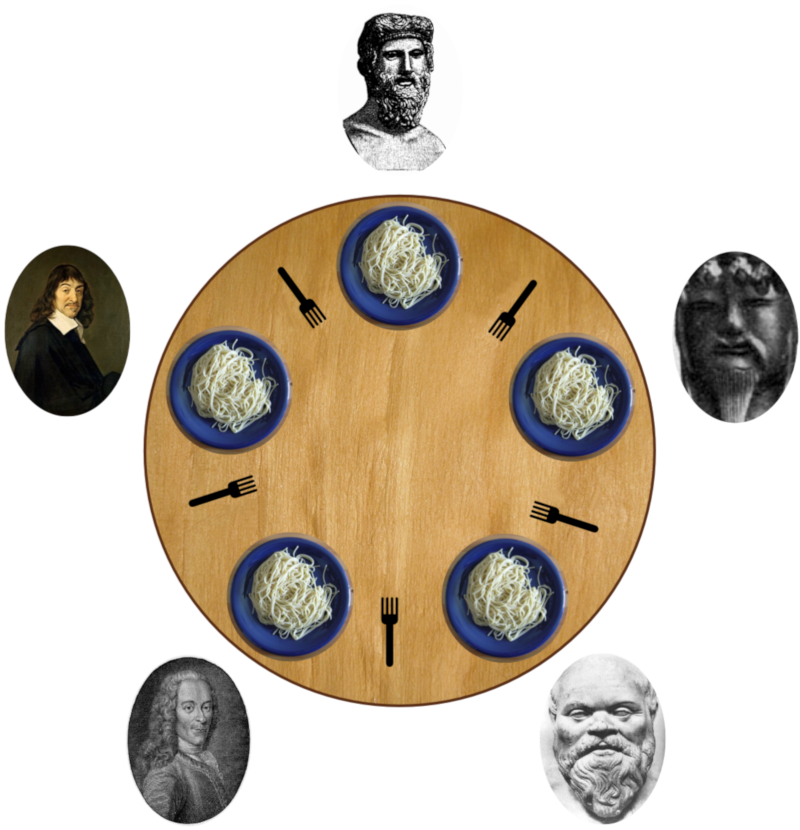
\includegraphics[width=6cm]{ressources/philo.png}
\captionof{figure}{Dîner des philosophes}
\label{philo}
\end{figure}
Le problème de circulation ci-dessous est un autre exemple classique.
\begin{figure}[!h]
\centering
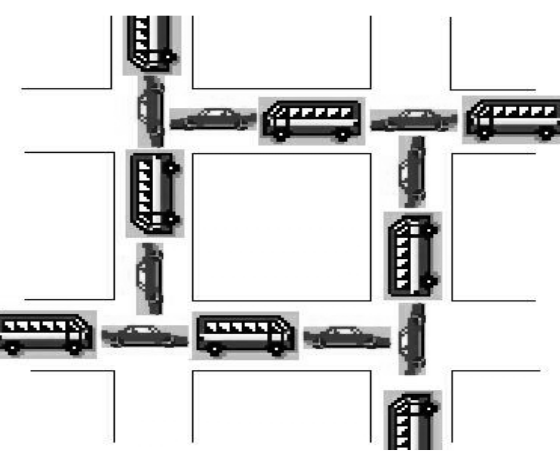
\includegraphics[width=6cm]{ressources/circulation.png}
\captionof{figure}{Circulation}
\label{circulation}
\end{figure}
\begin{center}
\textbf{Montrer que ces deux situations sont ou peuvent conduire à des interblocages.}
\end{center}
\end{Form}
\end{document}